
\chapter{Implementing the USB host stack}

The components of the USB host stack and their functions having been described in the previous chapter,
the implementation of the whole USB system is now elaborated on.
Amongst others, the directory structure, the API for the application, the drivers, 
the host controllers and the structure of the algorithm
for the subdivision of the I/O requests in transfer descriptors is described.
In the subchapter \glqq{}Integration in an own project\grqq{}(Page \pageref{integration}) is shown
what is important when integrating the USB stack in an own application.

\section{Features}
\index{USB-Stack}
The USB stack is to be flexibly applicable on most diverse processor architectures. 
Since the complete source code, including all the drivers, modules and libraries 
would be too big for an embedded system and most of it unnecessary for a project,
the stack was built in such a way that only the absolutely necessary parts can be
removed and connectet to each other.
\newline\newline
It has been tried to come to a compromise between simplicity and size of the source code.
For example, the USB device drivers are integrated dynamically in the stack, because 
several drivers can exist there at the same time. The host controller drivers,
on the other hand, are integrated statically in the program during the compilation, because
one single host controller is enough for an embedded system and thus less memory and program code
is needed for the management.
\newline\newline
The main features of the USB host stack are:
\begin{enumerate}
\item low memory usage (ca. 200 bytes)
\item small code size (starting with 4 KB)
\item modules and drivers are combinable flexibly
\item finished class and device drivers and libraries for USB devices
\item hub , mass storage , HID divers
\item uclibusb for USB device libraries (for example for the FT232)
\item simple host controller interface
\item already applicable on small 8 bit processors
\item all source codes are written in C
\end{enumerate}
In the next part, the subdivison of the single modules is observed.

\section{Module overview} \label{kap:moduluebersicht}
\index{Module}
By seperating the source code units skillfully it is possible to compilate
a stack only with parts that are absolutelly necessary.
In figure \ref{module_c} is shown how the single modules build up on each other and are depending on each other.

\begin{figure}[h]
{
\centering
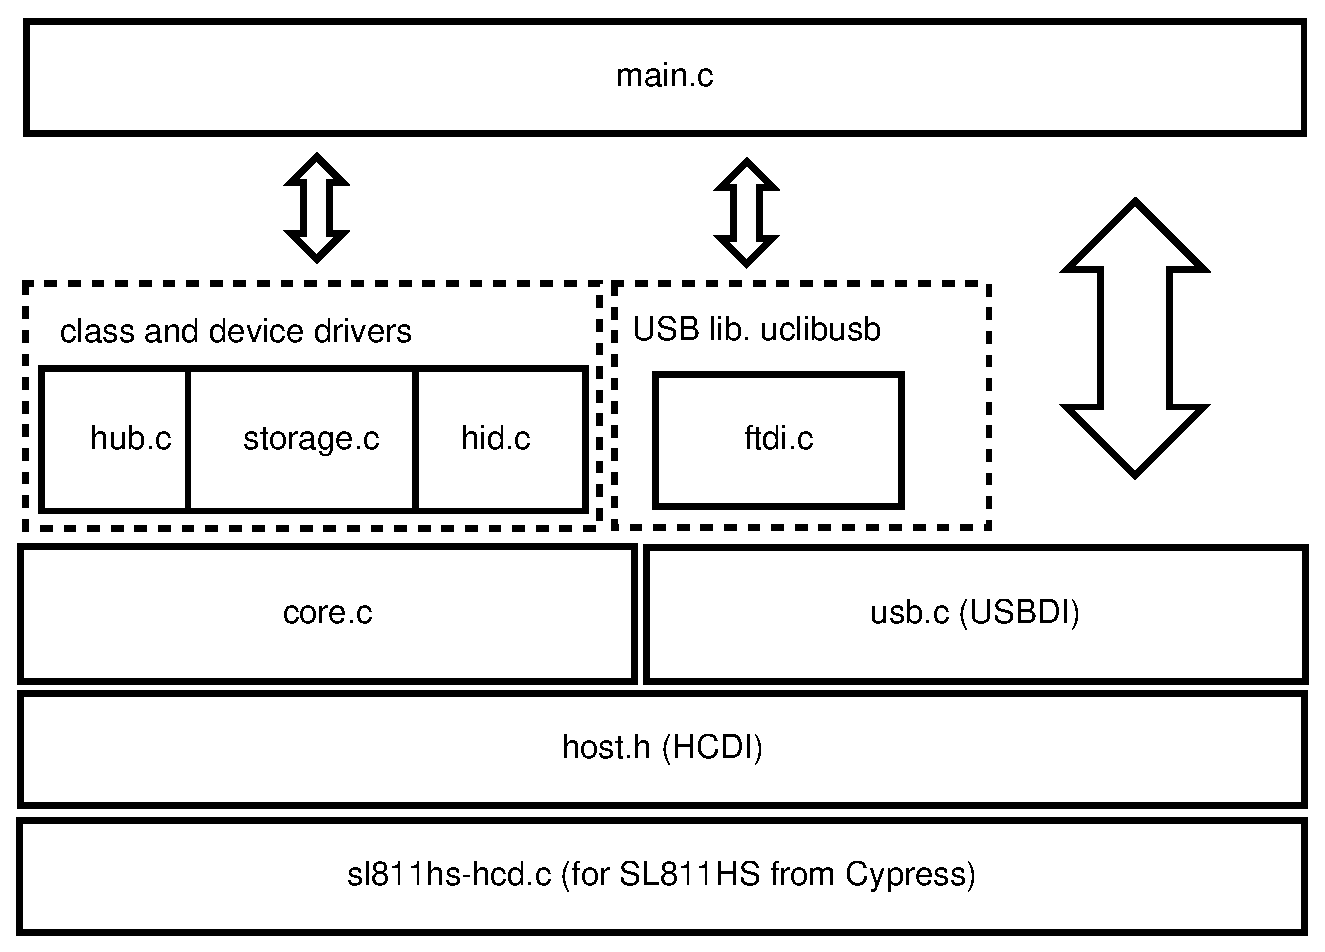
\includegraphics[width=11cm]{images/module_c}
\caption{C-modules of the USB stack}
\label{module_c}
}
\end{figure}
\index{Host-Controller-Treiber}
\index{Klassentreiber}
\index{Ger�tetreiber}
On the first level of the USB stack there is the host controller driver (e.g. \textbf{sl811hs-hcd.c} for the
host controller SL811HS from Cypress,
that has been inveted within the scope of this diploma thesis),
which has to provide the functions of the header file \textbf{host.h}.
With these functions, the USB stack can send and receive requests.
Furthermore, the functions for the root hub have to be integrated in the host controller driver (HCD).
In the file \textbf{core.c} are all functions for the management and the control
of the bus (drivers resp. device login and logout, etc.).
The USB stack provides the communication function for USB devices in the file \textbf{usb.c}.
\newline\newline
Besides the functions for a direct communication, there are also some drivers.
These drivers can be subdivided into two groups, the class and device drivers.
For devices for which no seperate drivers are required there is the possibility
to provide a library. Those are collected in the folder \textbf{uclibusb} - following the
concept of the well-known project libusb \cite{libusb}.

\section{Directory structure}
\index{Verzeichnisse}
The following directory structure was created for the USB Stack:

\begin{itemize} 
\item \textbf{arch} Example of an implementation for several microcontrollers
\item \textbf{boards} Circuit layout, PCB layout, etc. for the evaluation circuit
\item \textbf{core} USB core functions
\item \textbf{drivers} USB drivers (devices und classes)
\item \textbf{host} Host controller driver
%\item \textbf{hwmon} Hardware Monitor for the USB host controller 
\item \textbf{lib} Additional functions, type definitions, etc.
\item \textbf{uclibusb} USB libraries for USB devices
\item \textbf{usbspec} File types and formats of the USB specification
\item \textbf{doc} Doxygen documentation and the diploma thesis as a description
\end{itemize}


\section{Overview over the interfaces}
\index{API}
The APIs of the USB stack are subdivided into three groups (figure \ref{api}). 
In the lowest group the functions are defined, a host controller driver has to provide.
The second group forms the USB bus driver interface (USBDI) which provides functions for the communication 
of the device and driver management.
Finally, in the highest group the interface of an USB device resp. USB class driver is described.

\begin{figure}[h]
{
\centering
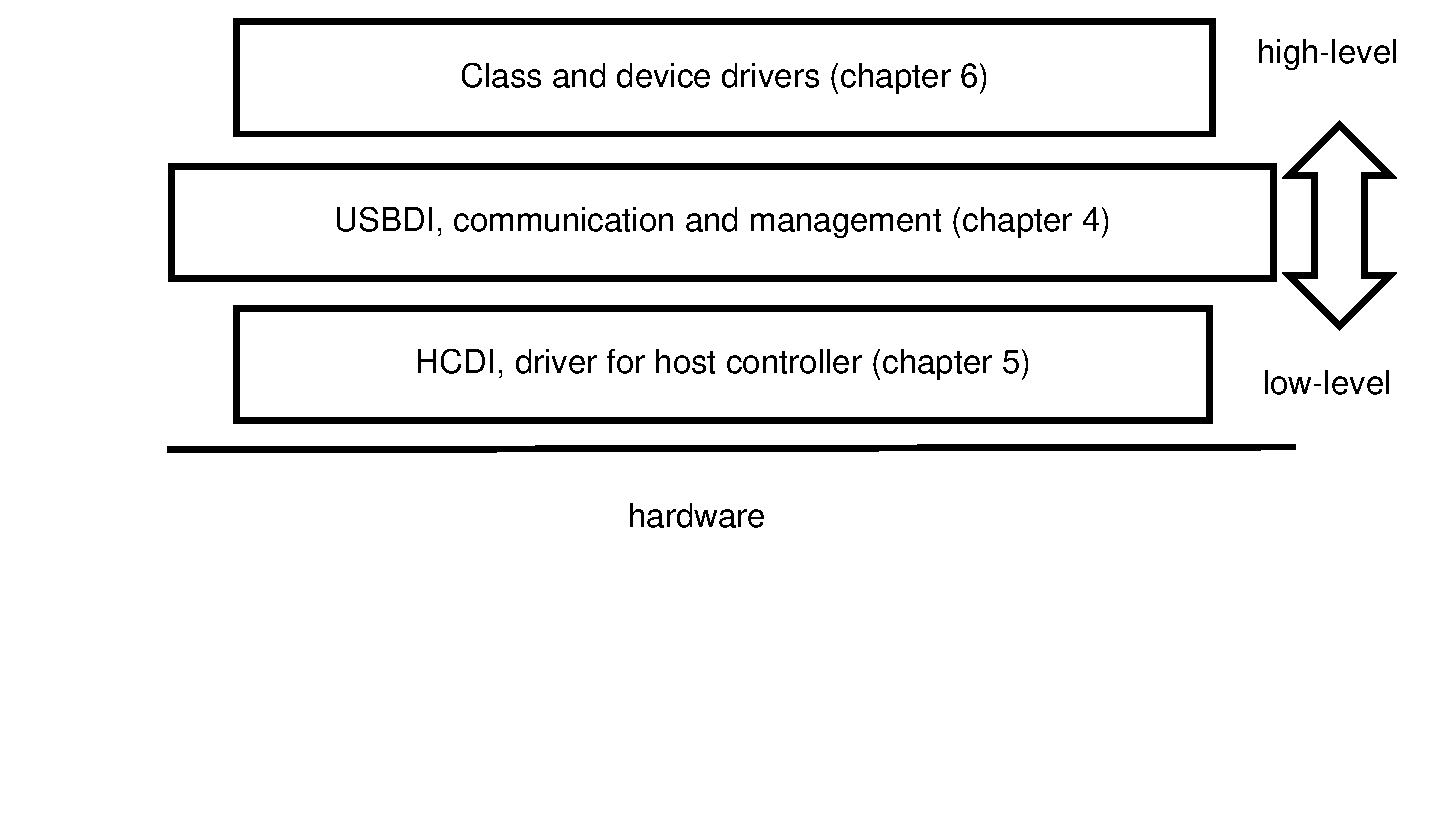
\includegraphics[width=15cm]{images/api}
\caption{USB stack interfaces}
\label{api}
}
\end{figure}
\subsection{HCDI (host controller driver interface)}
\index{Host-Controller-Treiber}
%Im Gegensatz zu einem USB-Ger�te-Treiber gibt es keine Datenstruktur f�r
%einen Host-Treiber, die dem USB-Stack �bergeben werden muss.
As already mentioned in the module overview (subchapter \ref{kap:moduluebersicht}),
a single host controller is sufficient for the connection of several USB devices.
Thatswhy the driver is linked statically to the program.
In order that the USB stack can access the host controller via the drivers, the following two functions 
have to be provided exactly like this.

\begin{table}[h]
\center
\begin{tabular}{|l|l|}
\hline
\rowcolor{Gray}[0.9\tabcolsep]
Function & Task\\ \hline
void hcdi\_init() & initiates host controller\\ \hline
u8 hcdi\_enqueue(usb\_transfer\_descriptor *td) & assigns transfer descriptor\\ \hline
%u8 hcdi\_dequeue(usb\_transfer\_descriptor *td) & �bertragung abbrechen \\ \hline
\end{tabular}
\caption{HCDI - host controller driver interface [host.h]}
\label{usb_device_add}
\end{table}
\index{host.h}
The initialization function is activated by the core right after the start.
Within it, host controller specific indexes can be declared correspondingly
so that the module is in an initialized state as well and can begin with its work.
Here often tasks arise like setting interrup masks, trigger reset processes, etc..
For the file tranfer described in chapter \ref{kap:datenuebertragung} on page \pageref{kap:datenuebertragung} 
the function \textit{hcdi\_enqueue} has to be implemented.
As parameter it gets pointer on transfer descriptors. A corresponding root hub driver
is responsible for the detection of new devices.
Further information on that in chapter \ref{{kap:roothub}} on page \pageref{kap:roothub}.


\subsection{USBDI (USB bus driver interface)}
\label{kap:usbdi}
\index{USB-Ger�te-Treiber}
\index{USBDI}
\index{USB-Bustreiber-Schnittstelle}
The structure of the USBDI API is similar to the GNU/Linux kernel \cite{kernel}
and the library libusb \cite{libusb}. On the one hand the developer benefits of it by 
becoming easier acquainted with the USB stack, when he already knows one of the both interfaces.
On the other hand, libraries can be developed on a computer and afterwards be integrated in the USB stack
with a few modulations.
\newline\newline
\textbf{Communication with devices}
\newline\newline
Before it is possible to access an USB device, a pointer to the device like \textit{usb\_device}
(see listing \ref{lst:usb_dev_struct}) is required.
\lstset{language=C}
\begin{lstlisting}[caption={USB device data structure, core.h},label={lst:usb_dev_struct},
captionpos=b,
basicstyle=\ttfamily\fontsize{10}{12}\selectfont,
commentstyle=\fontsize{10}{12}\selectfont]
typedef struct usb_device_t usb_device;
struct usb_device_t {
  /* Device information */
  u8  address;	     
  u8  fullspeed;
  /* USB device descriptor */
  u8  bMaxPacketSize0;
  u8  bDeviceClass;
  u8  bDeviceSubClass;
  u8  bDeviceProtocoll;
  u32 idVendor;
  u32 idProduct;
  u32 bcdDevice;
  u8  bNumConfigurations;
  /* End of USB device descriptor */

  /* Endpoint */
  u8 epSize[16];
  u8 epTogl[16];

  /* Pointer to the next device in the stack */
  usb_device *next;
};
\end{lstlisting}

This pointer is not an explicit \glqq{}handle\grqq{} to the device,
but a direct reference to the device data structure.
By using the functions \textit{usb\_open()} and \textit{usb\_open\_class()} (see table \ref{usb_device_add_open})
such a pointer can be detected.
If the device can't be found or if it is already reserved by anothter driver resp. process, you get a \textit{NULL}
as return value.
There is also the possibility to look for the device by yourself in the internal device lists of the USB core.
For further information on that, see chapter 6.
\newline\newline
When the requested device is found, files can be sent and received with the aid of the functions from table \ref{usb_uebertragung}.
As soon as the connection to the device isn't needed any more, calling the function {usb\_close} is enough to release
the device again for other applications or drivers.

\begin{table}[h]
\center
\begin{tabular}{|l|l|}
\hline
\rowcolor{Gray}[0.9\tabcolsep]
Function & Task\\ \hline
usb\_open(u32 vendor\_id, u32 product\_id) & finds device, manufacturer and product id\\ \hline
usb\_open\_class(u8 class) & finds device with class code\\ \hline
usb\_close(usb\_device *dev)  & closes connection to a device\\ \hline
\end{tabular}
\caption{USBDI - Opening a connection to the device [usb.h]}
\label{usb_device_add_open}
\end{table}

\begin{table}[h]
\center
\begin{tabular}{|l|}
\hline
\rowcolor{Gray}[0.9\tabcolsep]
Function \\ \hline
usb\_control\_msg(usb\_device *dev, char *buf, u8 size, u8 timeout) \\ \hline
usb\_control\_msg(usb\_device *dev, char *buf, u8 size, u8 timeout) \\ \hline
usb\_bulk\_write(usb\_device *dev, u8 ep, char *buf, u8 size, u8 timeout) \\ \hline
usb\_int\_read(usb\_device *dev, u8 ep, char *buf, u8 size, u8 timeout) \\ \hline
usb\_int\_write(usb\_device *dev, u8 ep, char *buf, u8 size, u8 timeout)  \\ \hline
usb\_isochron\_read(usb\_device *dev, u8 ep, char *buf, u8 size, u8 timeout)  \\ \hline
usb\_isochron\_write(usb\_device *dev, u8 ep, char *buf, u8 size, u8 timeout) \\ \hline
\end{tabular}
\caption{USBDI - Communication with the device [usb.h]}
\label{usb_uebertragung}
\end{table}
\index{usb.h}
Files can be transferred with the functions from the table \ref{usb_uebertragung}.
What the parameters of the functions stand for is described in the following:

\begin{itemize}
\item \textbf{usb\_device *dev} Pointer to the device
\item \textbf{u8 ep} Endpoint for the communication
\item \textbf{char *buf} Buffer for data to send and to receive
\item \textbf{u8 size} Number of files to send and to receive (in bytes)
\item \textbf{u8 timeout} Timeout after corrupted transfer (in milliseconds)
\end{itemize}
Contrary to the other transfer types no endpoint address has to be specified when using control transfer, because only
the endpoint 0 supports the control transfer.
There are also no seperate \glqq{}write\grqq{} and \glqq{}read\grqq{} functions, because 
only with the endpoint 0 data can be transfered bidirectionally.
\newline\newline
%Die vollst�ndige API-Dokumentation befindet sich im Anhang B.
\newpage
\textbf{Device management}
\index{Ger�teverwaltung}
\newline\newline
Another important part of the USB stack is the device management.
New devices have to be enumerated, data structures have to be created and plugged-out devices have to be removed again.
For those tasks, the USB stack provides the functions from the table \ref{usb_device_add_2}.

\begin{table}[h]
\center
\begin{tabular}{|l|l|}
\hline
\rowcolor{Gray}[0.9\tabcolsep]
Functions & Tasks\\ \hline
usb\_device * usb\_add\_device() & adds new device\\ \hline 
void usb\_remove\_device(usb\_device *dev) & removes new device\\ \hline 
\end{tabular}
\caption{Adding and removing a new device [core.h]}
\label{usb_device_add_2}
\end{table}
\index{core.h}
This function should only be called by hub and root hub drivers,
because only they can monitor the status of a port. 
When the hub detects an alteration (connection and disconnection of a device) on a port, the stack can be informed
with this function.
\newline\newline
\textbf{Driver management}
\index{Treiberverwaltung}
\newline\newline
The driver management provides the possibilty to add and remove drivers 
dynamically during runtime (see table \ref{usb_device_add})
When a new device is connected, the USB stack passes through the driver list
and calls a function from every driver to check if the new device is controllable by the driver.
A driver is represented in the system by the data structure \textit{usb\_driver *driver} (see listing \ref{lst:usb_driver}).
What parameters this structure contains exactly and what tasks they perform is described in the next subchapter.

\label{kap:usbdi_driver}
\begin{table}[h]
\center
\begin{tabular}{|l|l|}
\hline
\rowcolor{Gray}[0.9\tabcolsep]
Functions & Tasks\\ \hline
u8 usb\_register\_driver(usb\_driver *driver) & registers driver\\ \hline 
u8 usb\_unregister\_driver(usb\_driver *driver) & unregisters driver\\ \hline 
\end{tabular}
\caption{Registering and unregistering a driver [core.h]}
\label{usb_device_add}
\end{table}

\subsection{Class and device driver interface}
\index{Klassentreiber}
\index{Ger�tetreiber}
In order to register USB device drivers on the USB stack, an instance of 
the data structure \textit{usb\_driver} is needed.
In the data structure the name of the driver, the pointer \textit{probe}, including the address to the \glqq{}checking function\grqq{}
for newly detected devices and the pointer \textit{check}, including the address to a function for periodic management
and control tasks are specified.
Further information on the purpose of these functions is given in chapter 6.

\lstset{language=C}
\begin{lstlisting}[caption={USB driver data structure, core.h},label={lst:usb_driver},
captionpos=b,
basicstyle=\ttfamily\fontsize{10}{12}\selectfont,
commentstyle=\fontsize{10}{12}\selectfont]
usb_driver <driver name> = {
  .name   = "<driver name>",
  .probe  = usb_<driver name>_probe,
  .check  = usb_<driver name>_check,
  .data   = NULL
};
\end{lstlisting}
\begin{table}[h]
\center
\begin{tabular}{|l|l|}
\hline
\rowcolor{Gray}[0.9\tabcolsep]
Function & Task\\ \hline
void usb\_$<$treibername$>$\_init() & initializes driver \\ \hline
void usb\_$<$treibername$>$\_probe() & checks if there is a driver for the new device \\ \hline
void usb\_$<$treibername$>$\_check() & driver management and control\\ \hline
\end{tabular}
\caption{Device and class driver interface}
\label{usb_device_add_driver}
\end{table}


\section{Realization of the host communication}
The basis for this section forms chapter \ref{kap:datenuebertragung} on page \pageref{kap:datenuebertragung}.
There, the strategies for the data transfer with the host controller are described.
Thus, in the following sections only the implementation of the software structure for these strategies will be discussed.

\subsection{I/O request package (IRP)}
\index{I/O-Request-Paket}
An IRP (see listing \ref{irp_usb_2}) includes all the information for an USB request, such as the device address,
the endpoint, the transfer type, the number of bytes to receive and to send, and a pointer to a memory for the data.
The pointer \textit{usb\_transfer\_descriptor *head} points to the first transfer descriptor of the current IRP.

\lstset{language=C}
\begin{lstlisting}[caption={IRP data structure, core.h},label={irp_usb_2},
captionpos=b,
basicstyle=\ttfamily\fontsize{10}{12}\selectfont,
commentstyle=\fontsize{10}{12}\selectfont]
typedef struct usb_irp_t usb_irp;
struct usb_irp_t {
  usb_device * dev;   /* Pointer to the device structure */
  u8 endpoint;	      /* Endpoint + direction (bit 7) */
  u8 epsize;	      /* Size of the endpoint */
  
  u8 type;	      /* Transfer type */
  char * buffer;      /* Buffer for the transfer */
  u16 len;	      /* Number of data to transfer */

  usb_transfer_descriptor *head;  /* Pointer to the first TD */
  u16 timeout;	      /* Abandonment after x ms on error */
};
\end{lstlisting}
\index{core.h}
\subsection{Transfer descriptors (TD)}
\index{Transfer-Deskriptor}
A transfer descriptor (see listing \ref{usb_td_2}) describes a single USB package.
Joint transfer descriptors of an I/O request are interlinked with the pointers \textbf{usb\_transfer\_descriptor *next}.
Thereby it can be signalized when a complete I/O request is executed,
namely if and only if the last transfer descriptor from the chain has a \textit{NULL} in the pointer \textit{next}.

\lstset{language=C}
\begin{lstlisting}[caption={Transfer descriptor data structure, core.h},label={usb_td_2},
captionpos=b,
basicstyle=\ttfamily\fontsize{10}{12}\selectfont,
commentstyle=\fontsize{10}{12}\selectfont]
typedef struct usb_transfer_descriptor_t usb_transfer_descriptor;
struct usb_transfer_descriptor_t {
  u8 devaddress;  /* device addressGer�teadresse */
  u8 endpoint;	  /* endpoint */

  u8 pid;	  /* USB package type */
  u8 iso;	  /* isochronal transfer? */
  u8 togl;	  /* togl bit (DATA0 or DATA1) */

  char * buffer;  /* buffer for the transfer */
  u16 actlen;	  /* number of data to transfer */

  u8 state;	  /* state of the request */
  usb_transfer_descriptor *next;  /* pointer to the next TD */
  usb_irp * irp;  /* pointer to IRP */
};
\end{lstlisting}

In the next section the algorithm is described that is responsible for the subdivision of the I/O request packages in
transfer descriptors.

\subsection{Algorithm for the subdivision of an IRP in single TDs}

The basis for the subdivision of the I/O request packages is the process chart in figure \ref{fluss_control}.
With the aid of the control transfer it is described, how transfer descriptors can be created.
The subdivision for bulk, interrupt and isochronal transfer is similar to the control transfer.
The algorithm is implemented in the function \textit{usb\_submit\_irp(usb\_irp *irp)} for all transfer types.

\begin{figure}[h]
{
\centering
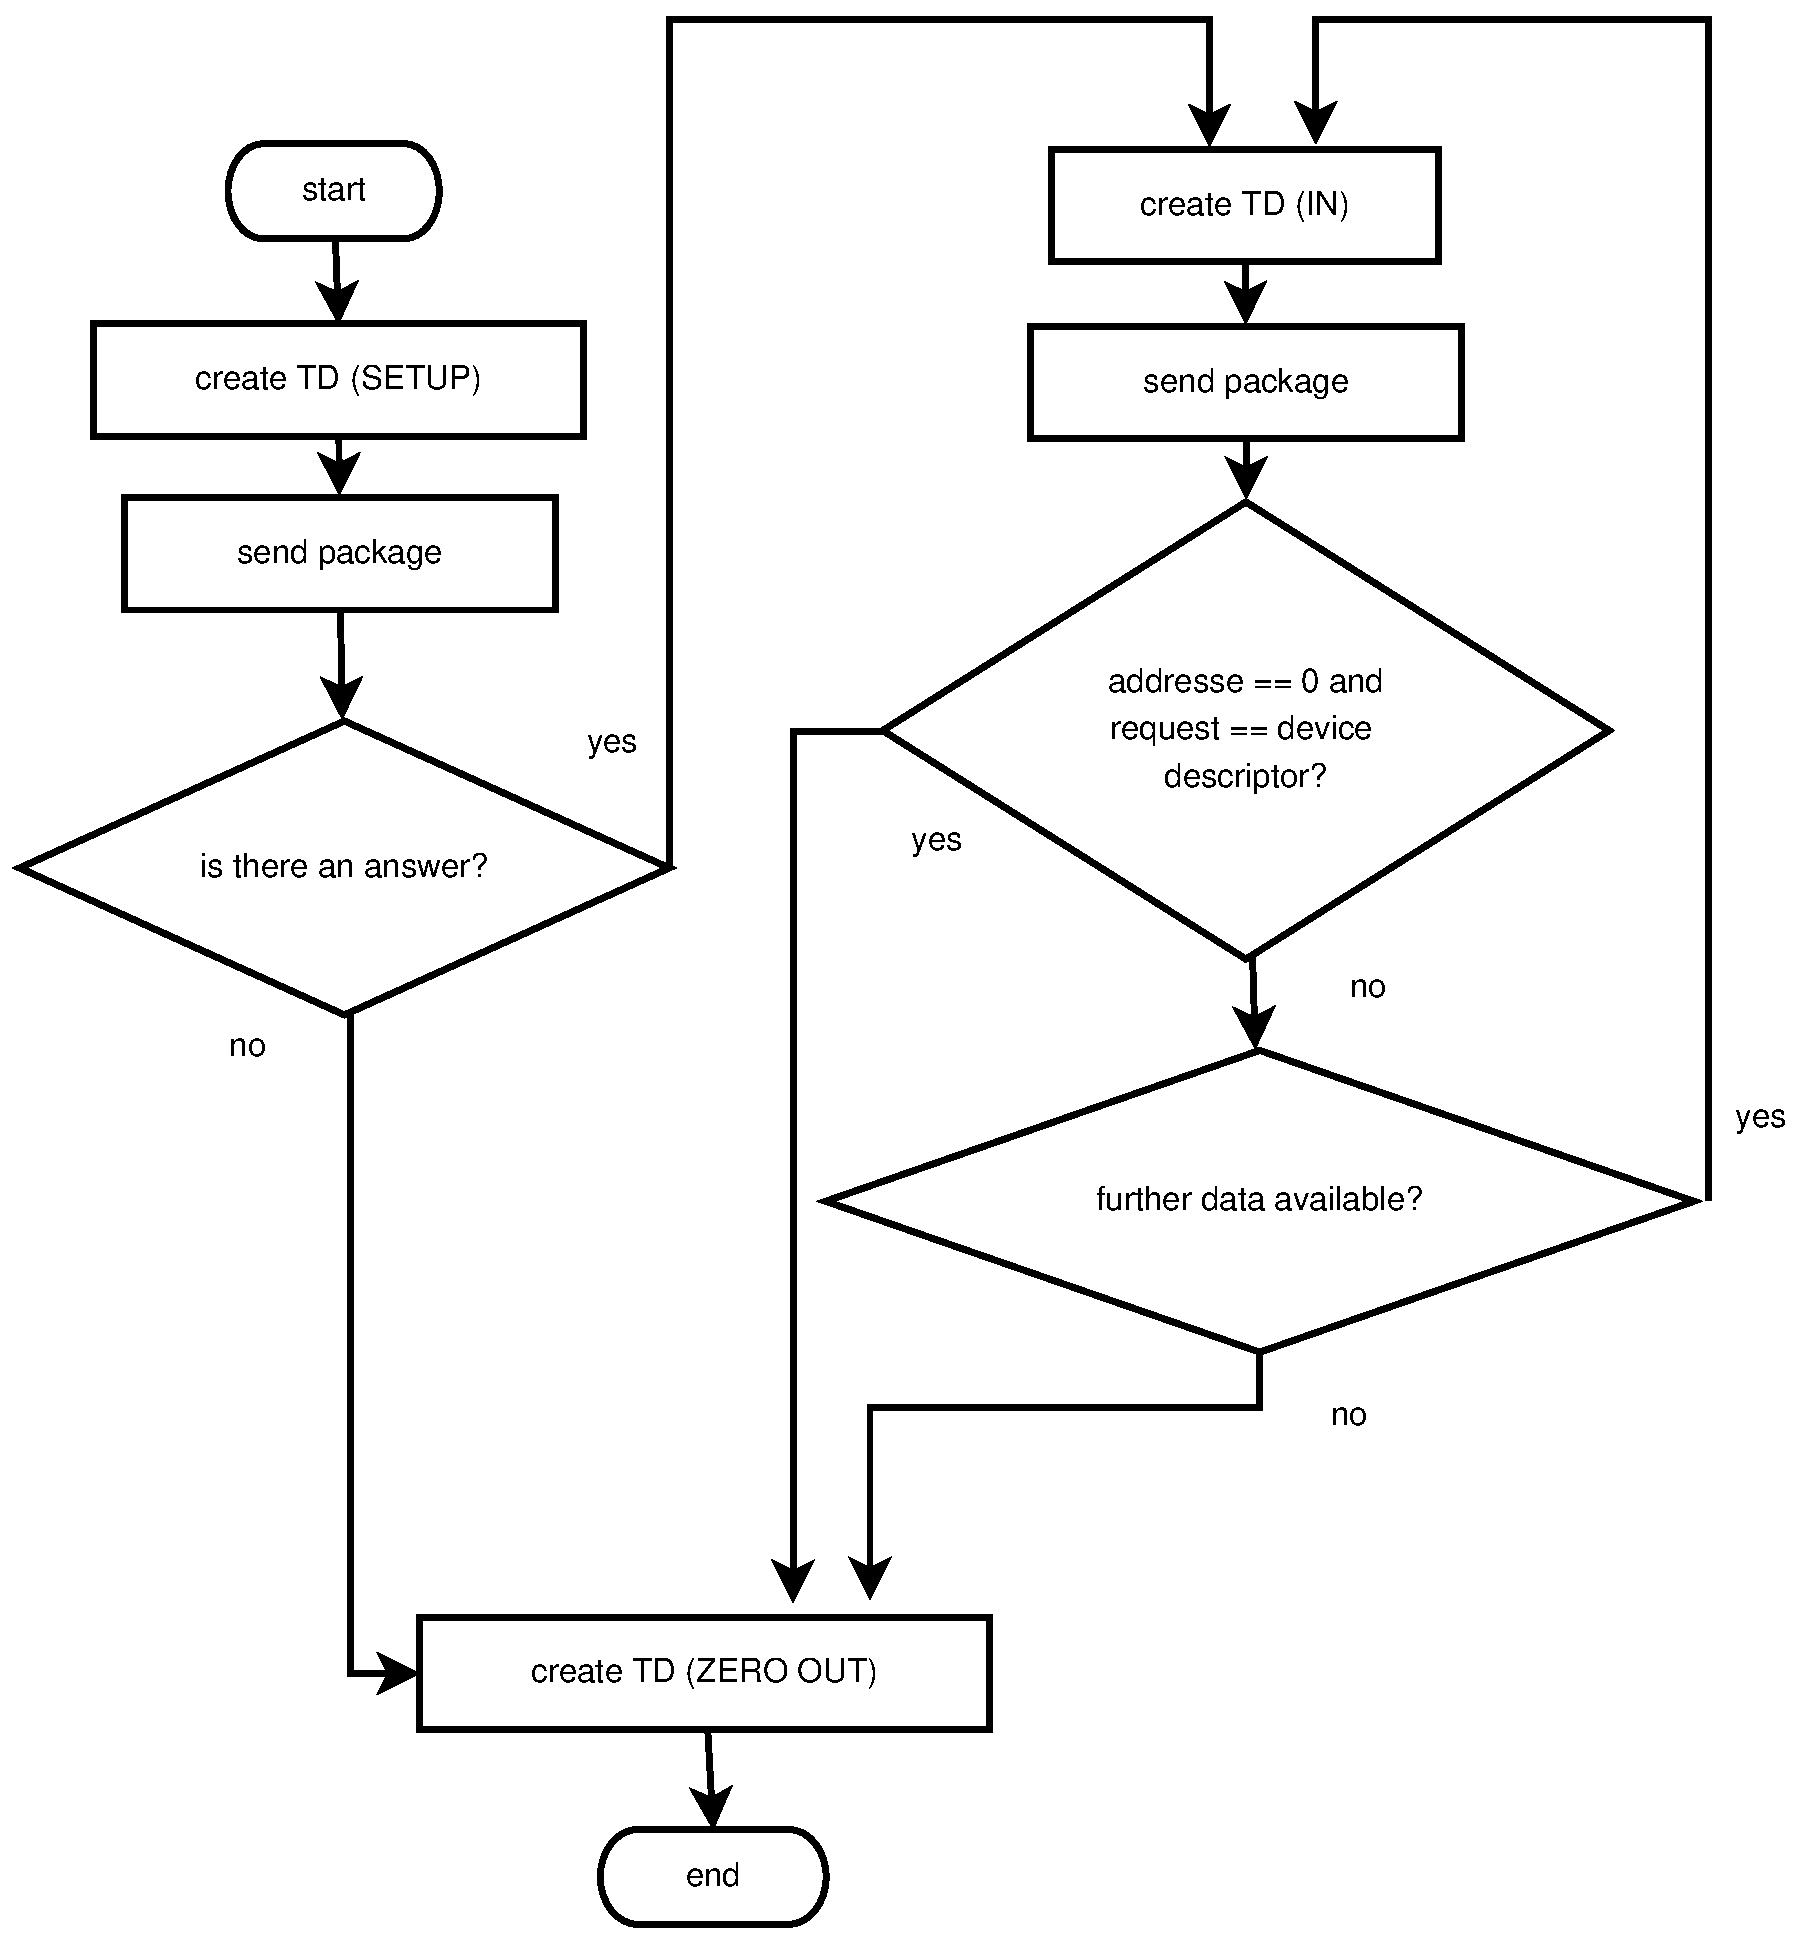
\includegraphics[width=12cm]{images/fluss_control}
\caption{Subdivision of a control transfer into transfer descriptors}
\label{fluss_control}
}
\end{figure}




\section{Integration in an own project}\label{integration}

In the following manual is described step by step how to integrate the USB stack in an existing or new project.
\newline\newline

\textbf{Step 1. Copy the USB directories} \newline
\newline
At first, the entire directories \textbf{core}, \textbf{lib} and \textbf{usbspec} are to be copied from the
USB stack archive to the own project directory.
If an own subfolder shall be created for the USB stack, the directories have to be copied
correspondingly to this folder.
\newline

\textbf{Step 2. Choose the host driver} \newline
\newline
In the next step a folder \textbf{host} is to be created on the same level as the folders in step 1.
In this folder a matching USB host controller driver has to be chosen from the archive and has to be copied to it.
For the compilation, the file \textbf{host.h} is also needed, thatswhy it has to be copied there aswell.
Many times, a driver needs additional files, for example the SL811HS driver.
There is another \textbf{sl811hs.h} file, that needs to be copied aswell.
If the host controller isn't integrated in the microprocessor, the connection and the transfer between microcontroller
and host controller is to be described, too.
In this case, the host controller provides own functions that, however, have to be adjusted.
How the connection is executed exactly has to be learned from the documentation of the host controller driver.
For the SL811HS this is described in chapter 8 of the diploma thesis.
\newline

\textbf{Step 3. Choose the drivers and the libraries }\newline
\newline
Exactly like the host driver, the necessary device drivers and libraries have to be copied in the created directory.
It is recommended to create the directory structure exactly as in the USB stack archive.
\begin{itemize}
\item drivers 
  \begin{itemize}
    \item class  
    \item net
    \item ...
  \end{itemize}
\item uclibusb
\end{itemize}

There are some folders, which are empty in the USB stack archive. Hopefully, after some time the collections grows bigger
and bigger.
\newline

\textbf{Step 4. Integrate the source codes in the compilation process} \newline
\newline
In the next step, the files have to be integrated in the compilation process of the project.
The directory including the USB stack files are to be given as include path, so that the compiler finds the
needed header files.
The command for the gcc would be \textit{gcc -I./}, or if there is an extra 
folder for the USB stack, \textit{gcc -I./foldertothestack}.
With the pre-processor flag DEBUG the debug mode can be switched on and off 
(\textit{gcc -DDEBUG=1} oder \textit{gcc -DDEBUG=0}).
\newline

\textbf{Step 5. Implementing the USB stack} \newline
The main function calls are shown in listing \ref{lst:usb_sample}.
In lines 1-4 the most important header files are integrated.
Which ones are to stand there depends on the drivers that are needed for the application.
The USB stack is initialized with the function call in line 8
Again, depending on the needed drivers the initialization functions of the drivers have to be called (lines 10-11).
For management and control tasks the USB stack has to be called regularly.
This can be solved with an infinite loop (line 13), or with a periodic timer of a thread library, etc.
If no periodic transfers happen and if the USB devices aren't changed during the operation,
periodic function calls can be foregone.

\lstset{language=C}
\begin{lstlisting}[caption={Implementing the USB stack},label={lst:usb_sample},
captionpos=b,
numbers=left,
basicstyle=\ttfamily\fontsize{10}{12}\selectfont,
commentstyle=\fontsize{10}{12}\selectfont]
#include <core/core.h>
#include <host/host.h>
#include <drivers/class/hub.h>
#include <drivers/class/storage.h>

int main(void)
{
  usb_init();

  usb_hub_init();
  usb_storage_init();
  
  while(1){
    usb_periodic(); 
    wait_ms(1);
  }
  return 0;
}
\end{lstlisting}

\textbf{Step 6.  Writing USB programs} \newline
The basis is now established and the programming of an USB application can be started.
A communication with an USB device, controlled directly by the functions of the USBDI may look like this:

\lstset{language=C}
\begin{lstlisting}[caption={Example of an USB program},label={lst:usb_driver_999},
captionpos=b,
numbers=left,
basicstyle=\ttfamily\fontsize{10}{12}\selectfont,
commentstyle=\fontsize{10}{12}\selectfont]
/* Pointer to the device data structure */
usb_device * dev = NULL;
char buf[] = {'A','B','C'};

/* Open USB connection to the device */
dev = usb_open(0x1234,0x5678);

/* Send data to the endpoint */
usb_bulk_write(dev,2,buf,3,1000);

/* Read data from the endpoint */
usb_bulk_read(dev,1,buf,3,1000);

/* Close connection */
usb_close(dev);

\end{lstlisting}
\index{Beispielprogramm}

%\section{Portierung auf eine neue Architektur}

%datentypen

%port leitungen fuer die hostcontroller treiber



%\section{USB Debug Monitor}
%\subsection{Integration in USB Host Stack}
%\subsection{Datenverkehr aufzeichnen}


